\documentclass{article}
\usepackage[utf8]{inputenc}
\usepackage[T1]{fontenc}
\usepackage{fancyhdr}
\usepackage{newpxtext,newpxmath} % Palatino font
\usepackage{lipsum} % For placeholder text
\usepackage{geometry}
\usepackage{tikz}
\usetikzlibrary{shapes.geometric, arrows, positioning, fit}

% --- Page Layout Configuration ---
\geometry{a4paper, margin=2.5cm}
\pagestyle{fancy}
\fancyhf{} % Clear all header and footer fields
\fancyhead[L]{Universidad Distrital Francisco José de Caldas}
\fancyhead[R]{IO I}
\renewcommand{\headrulewidth}{0.4pt}

% --- Document Information ---
\title{Propuesta de Proyecto Final: Sistema de Optimización Ferroviaria}
\author{Grupo 3}
\date{\today}

% --- Document Body ---
\begin{document}

\maketitle
\thispagestyle{fancy} % Apply fancy style to the title page as well

\tableofcontents
\newpage

\section{Planteamiento del Problema y Contexto}
La optimización de la cadena de suministro es un desafío crítico para cualquier empresa de logística, y el transporte ferroviario no es una excepción. Este proyecto aborda un problema dual que enfrenta una compañía ferroviaria, combinando decisiones estratégicas de distribución con decisiones operativas de carga para maximizar la eficiencia y rentabilidad.

El objetivo es desarrollar un sistema de soporte a la decisión que resuelva dos problemas fundamentales y complementarios de la Investigación de Operaciones:

\begin{enumerate}
    \item \textbf{Problema de Transporte (Nivel Estratégico):} La compañía posee varios centros de distribución (orígenes) con una oferta limitada de un producto y debe abastecer a diferentes ciudades (destinos) que tienen una demanda específica. El objetivo es determinar el plan de envío óptimo, es decir, cuántas unidades de producto enviar desde cada origen a cada destino para satisfacer toda la demanda al menor costo de transporte total posible.
    \item \textbf{Problema de Carga (Nivel Operativo):} Para un viaje concreto entre un origen y un destino, el tren tiene una capacidad de carga limitada. La compañía dispone de un conjunto de mercancías heterogéneas que puede transportar, cada una con un peso (o volumen) y un beneficio asociado diferente. El objetivo es seleccionar qué conjunto de mercancías cargar en el tren para maximizar el beneficio total de ese viaje, sin exceder su capacidad.
\end{enumerate}

La solución integrada de estos dos problemas permite a la empresa no solo diseñar una estrategia de distribución de bajo costo, sino también maximizar la rentabilidad de cada operación individual. El sistema propuesto aplicará dos métodos clave vistos en la asignatura para modelar y resolver cada uno de estos desafíos.

\section{Formulación Matemática}
Para abordar el problema dual, lo descomponemos en dos modelos matemáticos, cada uno resuelto con una técnica de optimización apropiada.

\subsection{Modelo de Transporte (Método de Vogel)}
El problema de minimizar el costo de distribución se modela como un \textbf{Problema de Transporte}. Este es un caso particular de la Programación Lineal.

\begin{itemize}
    \item \textbf{Índices y Conjuntos:}
        \begin{itemize}
            \item $i \in \{1, ..., m\}$: Conjunto de orígenes (centros de distribución).
            \item $j \in \{1, ..., n\}$: Conjunto de destinos (ciudades).
        \end{itemize}
    \item \textbf{Parámetros:}
        \begin{itemize}
            \item $O_i$: Oferta o capacidad de producción del origen $i$.
            \item $D_j$: Demanda del destino $j$.
            \item $C_{ij}$: Costo de transportar una unidad desde el origen $i$ al destino $j$.
        \end{itemize}
    \item \textbf{Variables de Decisión:}
        \begin{itemize}
            \item $X_{ij}$: Cantidad de unidades a enviar desde el origen $i$ al destino $j$.
        \end{itemize}
\end{itemize}

\textbf{Función Objetivo (a minimizar):}
$Z = \sum_{i=1}^{m} \sum_{j=1}^{n} C_{ij} X_{ij}$

\textbf{Sujeto a las restricciones:}
\begin{align*}
    \sum_{j=1}^{n} X_{ij} &\leq O_i \quad \forall i \in \{1, ..., m\} \quad \text{(Restricciones de Oferta)} \\
    \sum_{i=1}^{m} X_{ij} &\geq D_j \quad \forall j \in \{1, ..., n\} \quad \text{(Restricciones de Demanda)} \\
    X_{ij} &\geq 0 \quad \forall i, j
\end{align*}

Para este proyecto, se implementará el \textbf{Método de Aproximación de Vogel} para encontrar una solución básica factible inicial de alta calidad. Este método heurístico es a menudo superior a otros métodos iniciales (como Esquina Noroeste o Costo Mínimo) porque considera los "costos de penalización" por no elegir las rutas más baratas, lo que generalmente conduce a una solución inicial más cercana a la óptima.

\subsection{Optimización de Carga (Programación Entera Pura)}
Una vez que se ha decidido realizar un envío desde un origen $i$ a un destino $j$, se presenta el problema de seleccionar la carga óptima. Este es un ejemplo clásico del \textbf{Problema de la Mochila 0/1} (0/1 Knapsack Problem) y se resuelve utilizando Programación Entera Pura.

\begin{itemize}
    \item \textbf{Índices y Conjuntos:} Sea $N = \{1, 2, ..., n\}$ el conjunto de tipos de mercancías disponibles para ser transportadas.
    \item \textbf{Parámetros:}
        \begin{itemize}
            \item $p_i$: El beneficio o ganancia monetaria obtenida por transportar una unidad de la mercancía $i$.
            \item $w_i$: El peso (o volumen) de una unidad de la mercancía $i$.
            \item $C$: La capacidad máxima total de carga del tren.
        \end{itemize}
    \item \textbf{Variables de Decisión:}
        \begin{itemize}
            \item $x_i$: Una variable binaria que toma el valor de 1 si la mercancía $i$ es seleccionada para ser transportada, y 0 en caso contrario.
            \item $x_i \in \{0, 1\}$ para $i \in N$.
        \end{itemize}
\end{itemize}

\textbf{Función Objetivo:}
Maximizar $Z = \sum_{i=1}^{n} p_i x_i$

\textbf{Sujeto a la restricción:}
$\sum_{i=1}^{n} w_i x_i \leq C$

Este modelo matemático asegura que se maximice el beneficio total sin exceder la capacidad de carga del tren. La naturaleza binaria de las variables de decisión ($x_i$) lo clasifica como un problema de Programación Entera Pura.

\section{Arquitectura del Software}

\begin{figure}[h!]
\centering
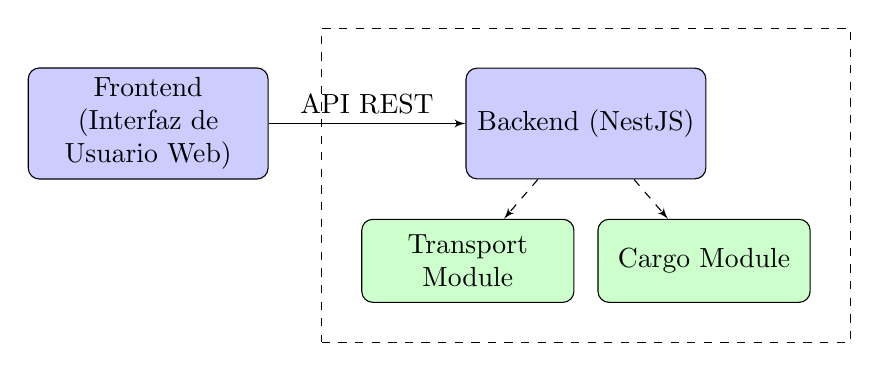
\begin{tikzpicture}[
    node distance=1.5cm and 2.5cm,
    block/.style={rectangle, draw, fill=blue!20, text width=8em, text centered, rounded corners, minimum height=4em},
    subblock/.style={rectangle, draw, fill=green!20, text width=7em, text centered, rounded corners, minimum height=3em},
    line/.style={draw, -latex'}
]
    % Nodes
    \node[block] (frontend) {Frontend (Interfaz de Usuario Web)};
    \node[block, right=of frontend] (backend) {Backend (NestJS)};

    % Backend internal modules
    \node[subblock, below=0.5cm of backend, xshift=-1.5cm] (transport) {Transport Module};
    \node[subblock, below=0.5cm of backend, xshift=1.5cm] (cargo) {Cargo Module};

    % Dashed box for backend
    \node[draw, dashed, fit=(backend) (transport) (cargo), inner sep=0.5cm] (backend-box) {};

    % Arrows
    \path[line] (frontend) -- node[midway, above] {API REST} (backend);
    \path[line, dashed] (backend) -- (transport);
    \path[line, dashed] (backend) -- (cargo);

\end{tikzpicture}
\caption{Diagrama de la arquitectura del software propuesto.}
\label{fig:arquitectura}
\end{figure}

Para el desarrollo del sistema interactivo, se propone una arquitectura de software moderna y desacoplada, como se muestra en la Figura~\ref{fig:arquitectura}. Esta se basa en un backend robusto y un frontend dinámico. La tecnología principal para el servidor será \textbf{NestJS}, un framework de Node.js que utiliza TypeScript y promueve una estructura modular y escalable, inspirada en Angular.

La arquitectura se dividirá en dos componentes principales:

\begin{enumerate}
    \item \textbf{Backend (Servidor):}
    Desarrollado con NestJS, será el cerebro de la aplicación y el responsable de toda la lógica de negocio y los cálculos de optimización. Su estructura interna se organizará en los siguientes módulos:
    \begin{itemize}
        \item \textbf{Controlador de API (API Controller):} Será el punto de entrada, exponiendo endpoints RESTful para que el frontend envíe los datos de los problemas. Recibirá la matriz de costos, los vectores de oferta/demanda y los datos de las mercancías, y devolverá las soluciones consolidadas.
        \item \textbf{Módulo de Transporte (Transport Module):} Contendrá un `TransportService` responsable de implementar la lógica del Método de Aproximación de Vogel. Recibirá los datos del problema de transporte y devolverá la matriz de asignación inicial que minimiza los costos.
        \item \textbf{Módulo de Carga (Cargo Module):} Incluirá un `CargoService` dedicado a resolver el problema de la mochila mediante un modelo de Programación Entera. Este servicio recibirá la lista de mercancías y la capacidad del tren, y devolverá la selección óptima. Podría usar una librería de optimización como `glpk.js`.
    \end{itemize}
    Esta separación de responsabilidades asegura que la lógica de cada problema de optimización esté aislada y sea fácil de mantener o mejorar en el futuro.

    \item \textbf{Frontend (Aplicación Web):}
    Será la interfaz gráfica con la que interactuará el usuario. Aunque el framework específico puede ser elegido posteriormente (e.g., React, Angular, Vue.js), su función será:
    \begin{itemize}
        \item Proporcionar formularios intuitivos para que el usuario pueda definir el problema: cargar la red de ciudades y distancias, la lista de mercancías, etc.
        \item Enviar los datos al backend a través de peticiones HTTP a la API RESTful.
        \item Recibir los resultados del backend (la ruta óptima y la carga seleccionada) y presentarlos de forma clara y visualmente atractiva, por ejemplo, dibujando el grafo con la ruta resaltada y mostrando una tabla con la carga óptima y el beneficio total.
    \end{itemize}
\end{enumerate}

Esta arquitectura cliente-servidor es flexible, escalable y permite que el desarrollo del frontend y el backend se realice de forma independiente.

\section{Resultados y Análisis}
\lipsum[6]

\section{Conclusiones y Recomendaciones}
\lipsum[7]

\end{document}